\section{Model}

The underlying unobserved trait is modelled by the random variable
\begin{align}\label{eq:lattrait}
  z = a + b + \epsilon
\end{align} where $a$ is the fixed-effect
component (also known as covariate effects), $b$ is the random-effect component,
and $\epsilon$ is the i.i.d. normally-distributed noise.
The fixed-effect is defined by a dot-product between a vector of covariates and
a vector of fixed-effect sizes:
\begin{align*}
  a = \mathbf a\Tr \boldsymbol\alpha.
\end{align*}
The random-effect is also defined by a dot-product but now between
a vector of stuff and a vector of random-effect sizes:
\begin{align*}
  b = \mathbf b\Tr \bbeta, \qquad \bbeta \sim \mathcal N(0, \sigma^2_{\beta})
\end{align*}

Finally, the i.i.d. noise $\epsilon$ is normally distributed with variance
$\sigma^2_{\epsilon}$.
Assuming independence, we have $\mathrm E[b_s] = 0$ and
$\mathrm V[b_s]=1/\sqrt{n_b}$ for $s \in \{1, \dots, n_b\}$.
The overall effect-size of the random component $b$ will be given by
$\mathrm V[b] = \sigma^2_{\beta}$.
Knowing the values of $\boldsymbol\alpha$ and making analogous
assumptions about the covariates leads to $\mathrm V[a]  =
\sum_{j=1}^{n_a} \alpha_j^2$.
We define the narrow-sense heritability
\begin{align*}
  h^2=\frac{\sigma^2_{\beta}}{\sigma_t^2}, \text{where} \qquad \sigma_t^2 =
  \sum_{j=1}^{n_a} \boldsymbol \alpha_j^2 + \sigma^2_{\beta} +
  \sigma^2_{\epsilon}
\end{align*}
is the variance of $z$.

The unobserved process we have described in Eq. \eqref{eq:lattrait} is assumed
to be directly associated with the observed one via a link function:
\begin{align*}
  g(\mathrm E[y|z]) = z.
\end{align*}
If the distribution of $y$, give $z$, is completely defined by its
expected value, we have now established the distribution of $y$ via
$p(y) = \int p(y|z)p(z)dz$.
Therefore the user is free to choose whatever distribution (conditioned on the
latent variable $z$) represents best the observed process.
Fig. \ref{fig:gm} shows the corresponding graphical model representation.

\begin{figure}[ht]\label{fig:gm}
  \centering
  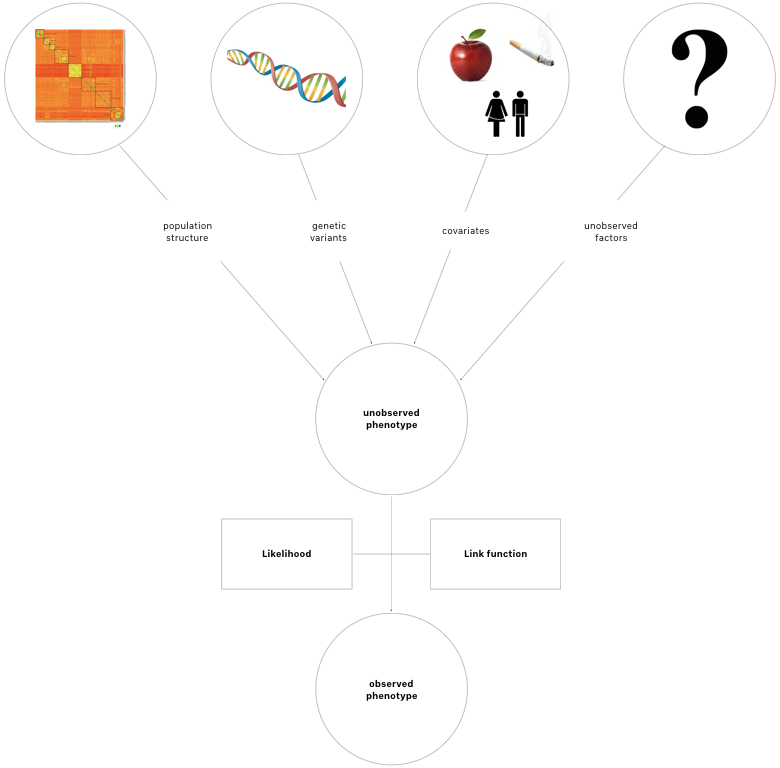
\includegraphics[width=0.5\textwidth]{images/friendly-model.png}
\end{figure}

\subsection{Example}

Let $y$ denotes the number of intron retentions out of $k$ mRNA reads.
One might regard $y$ as a Binomial random variable defined by $k$ number of
trials and an unknown probability of success $r$.
The relationship between $r$ and the genetic factors, environmental signal,
and noise can be established via a link function $g(\cdot)$ such that
$g(r)$ follows a latent process.
Here, we define such an unobserved process via Eq. \eqref{eq:lattrait}.
Precisely, we have
\begin{align*}
  p(y) = \int \Binom{y}{k}{g(r) = z} \Normal{z}{a}{\sigma^2_\beta + \sigma^2_\epsilon} dz.
\end{align*}
